\documentclass[10pt]{article}
\usepackage[polish]{babel}
\usepackage[utf8]{inputenc}
\usepackage[T1]{fontenc}
\usepackage{amsmath}
\usepackage{amsfonts}
\usepackage{amssymb}
\usepackage[version=4]{mhchem}
\usepackage{stmaryrd}
\usepackage{graphicx}
\usepackage[export]{adjustbox}
\graphicspath{ {./images/} }

\title{XIV Konkurs Matematyczny St@ś }

\author{}
\date{}


\begin{document}
\maketitle
\section*{XIV LO im. Stanisława Staszica}
2 czerwca 2014 roku

\section*{klasa V}
Na rozwiazanie poniższych zadań masz 90 minut. Kolejność rozwiazywania tych zadań jest dowolna. Wszystkie zadania sa jednakowo punktowane. Maksymalnq liczbę punktów mȯ̇e uzyskać jedynie petne rozwiazanie, z uzasadnieniem i odpowiedziq.\\
Używanie korektora i korzystanie z kalkulatora jest niedozwolone.

\begin{enumerate}
  \item Dany jest prostokąt \(A B C D\). Na jego bokach \(A B\) i \(B C\) zaznaczono punkty \(E\) i \(F\). Znamy długości odcinków: \(A E=2, E B=4, B F=6\) i \(F C=3\). Oblicz pole trójkąta \(D E F\).\\
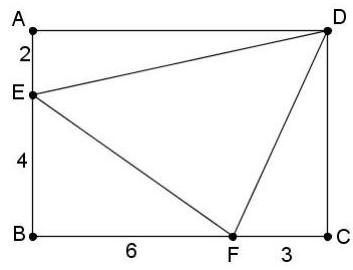
\includegraphics[max width=\textwidth, center]{2024_11_21_a8036543db8f2963a2e7g-1(1)}
  \item Cztery proste przecinające się w jednym punkcie dzielą płaszczyznę na osiem kątów. Trzy z nich mają miary: \(52^{\circ}, 94^{\circ}\) i \(16^{\circ}\). Jakie miary mają pozostałe kąty?
  \item Pewną liczbę podzielono przez 205 i otrzymano resztę 107. Jaką resztę otrzymamy jeśli podzielimy tę liczbę przez 5?
  \item Na rysunku widać ten sam sześcian widziany z różnej strony oraz jego siatkę. Wpisz w puste ściany siatki odpowiednie cyfry. Zdecyduj czy dana cyfra stoi normalnie, jest obrócona w prawo, w lewo czy może stoi "do góry nogami".\\
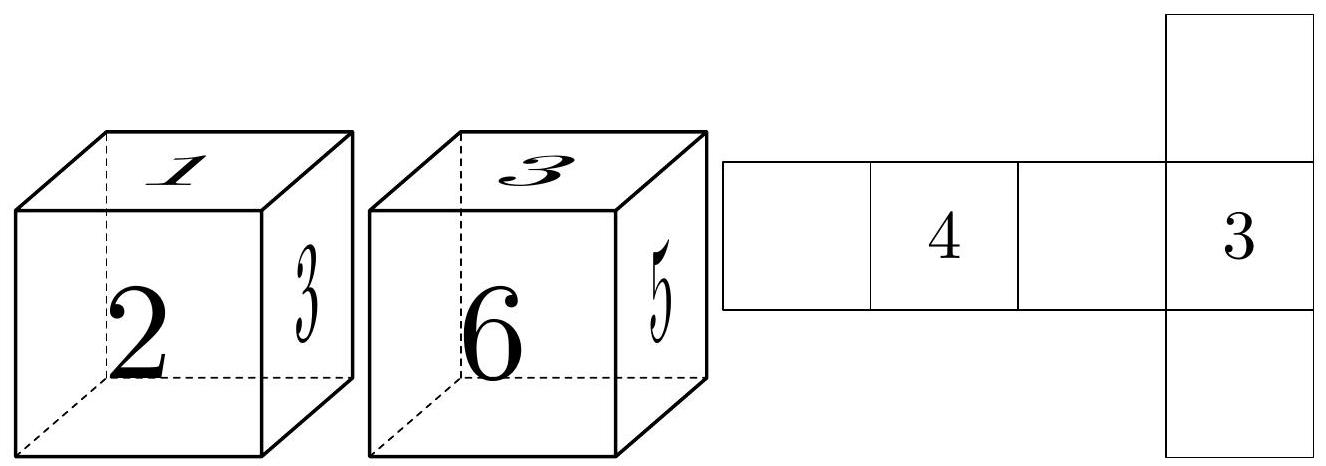
\includegraphics[max width=\textwidth, center]{2024_11_21_a8036543db8f2963a2e7g-1(2)}
  \item Wewnątrz każdego kwadratu wpisz jedną cyfrę tak, aby działanie było poprawne. Podaj jeden przykład.\\
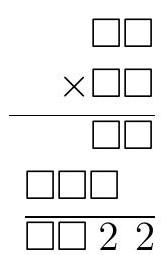
\includegraphics[max width=\textwidth, center]{2024_11_21_a8036543db8f2963a2e7g-1}
\end{enumerate}

\end{document}